\section{数据探索与可视化}
\subsection{数据探索}
数据集来自\href{http://capitalbikeshare.com/system-data}{capitalbikeshare}\cite{data}。\commandbox{hour.csv}数据集有17379条数据且无缺失,总共记录了17379小时;\commandbox{day.csv}数据集有731条数据且无缺失,总共记录了两年的单车使用状况。除了\verbbox[blue]{hr}维度不存在于\commandbox{day.csv}外,两个数据集都有以下的维度:
\begin{itemize}
    \item \verbbox[blue]{instant}::记录的索引
    \item \verbbox[blue]{dteday}:日期
    \item \verbbox[blue]{season}:季节(1至4分别代表春夏秋冬)
    \item \verbbox[blue]{yr}:年(0至1分别代表2011年与2012年)
    \item \verbbox[blue]{mnth}:月份(1至12)
    \item \verbbox[blue]{hr}:小时(0至23)
    \item \verbbox[blue]{holiday}:是否为节假日(根据\href{http://dchr.dc.gov/page/holiday-schedule}{\texttt{dc.gov}}网站)
    \item \verbbox[blue]{weekday}:该日是一周的第几天
    \item \verbbox[blue]{workingday}:是否为工作日
    \item \verbbox[blue]{weathersit}:天气情况(1至4分别代表晴天、多云、小雨、暴雨)
    \item \verbbox[blue]{temp}:标准化的摄氏度下温度(除以最大值41)
    \item \verbbox[blue]{atemp}:标准化的摄氏度下的体感温度(除以最大值50)
    \item \verbbox[blue]{hum}:标准化的湿度(除以最大值100)
    \item \verbbox[blue]{windspeed}:标准化的风速(除以最大值67)
    \item \verbbox[blue]{casual}:未注册用户的数量
    \item \verbbox[blue]{registered}:注册用户的数量
    \item \verbbox[blue]{cnt}:注册与未注册用户的总数量
\end{itemize}

从直观来说,共享单车的使用过程与周围的环境性与季节性的变化密切相关,例如天气的状态、降雨量、季节、一周内相对时间、一天内相对时间等。于是我们可以得到下述假设:
\begin{itemize}
    \item 天气晴朗适宜单车出行而阴雨不适宜;
    \item 温度舒适适宜单车出行而过低过高不适宜;
    \item 位于工作日由于上下班需求单车使用率高而周末出门游玩单车使用率可能也较高;
    \item 一天内上下班高峰期与中午时间单车使用率高而其他时间使用率相对较低。
\end{itemize}
因此我们使用时间相关的变量去预测注册用户与未注册用户的数量,同时使用环境相关的变量去预测注册用户与未注册用户的数量。我们可以将此问题看作回归问题,同时构造回归模型。

首先我们将数据集分为训练集与测试集,以此判断回归模型的好坏与避免模型的欠拟合与过拟合。按照规则,我们提取出每月前19天作为训练集,其余天数作为测试集。将除\verbbox[blue]{casual}、\verbbox[blue]{registered}与\verbbox[blue]{cnt}这三列的数据视做变量向量$\vecx$,将\verbbox[blue]{cnt}列视做响应向量$\vecy$。

其次我们计算出数据的描述性统计量,以此大致判断数据集的分布及形状。由表~\ref{T:train-day_x-data}、表与\ref{T:train-day_y-data}可以得出训练集的个数、均值、方差、最小最大值与分位数。部分列向量已经过归一化处理,不难看出数据基本不符合正态分布,同时由\verbbox[violet]{scipy.stats.kstest}计算可得出上述结论。

\begin{table}[htbp]
    \centering\tiny
    \begin{tabular}{lrrrrrrrrrrr}
    \toprule
    {} &  season &     yr &    mnth &  holiday &  weekday &  workingday &  weathersit &    temp &   atemp &     hum &  windspeed \\
    \midrule
    count &  456 &  -  &   -  &   -  &   -  &   -  &   -  &   -  &   -  &   -  &   -  \\
    mean  & 2.50 & 0.5 & 6.50 & 0.03 & 3.00 & 0.68 & 1.39 & 0.49 & 0.47 & 0.62 & 0.19 \\
    std   & 1.12 & 0.5 & 3.46 & 0.17 & 2.01 & 0.47 & 0.54 & 0.18 & 0.16 & 0.14 & 0.08 \\
    min   & 1.00 & 0.0 & 1.00 & 0.00 & 0.00 & 0.00 & 1.00 & 0.11 & 0.10 & 0.00 & 0.02 \\
    25\%  & 1.75 & 0.0 & 3.75 & 0.00 & 1.00 & 0.00 & 1.00 & 0.34 & 0.34 & 0.51 & 0.14 \\
    50\%  & 2.50 & 0.5 & 6.50 & 0.00 & 3.00 & 1.00 & 1.00 & 0.50 & 0.49 & 0.62 & 0.18 \\
    75\%  & 3.25 & 1.0 & 9.25 & 0.00 & 5.00 & 1.00 & 2.00 & 0.65 & 0.60 & 0.72 & 0.23 \\
    max   & 4.00 & 1.0 &12.00 & 1.00 & 6.00 & 1.00 & 3.00 & 0.86 & 0.80 & 0.97 & 0.51 \\
    \bottomrule
    \end{tabular}
    \cprotect\caption{\commandbox{day.csv}训练集变量数据探索}\label{T:train-day_x-data}
\end{table}

\begin{table}[htbp]
    \centering\tiny
    \begin{tabular}{lrrr}
    \toprule
    {}    &  casual & registered &  cnt \\
    \midrule
    count &    456  &     -   &     -   \\
    mean  &  859.95 & 3713.47 & 4573.41 \\
    std   &  698.91 & 1494.48 & 1868.74 \\
    min   &    9.00 &  491.00 &  605.00 \\
    25\%  &  318.00 & 2696.00 & 3305.50 \\
    50\%  &  722.00 & 3700.00 & 4585.50 \\
    75\%  & 1141.75 & 4814.25 & 5987.50 \\
    max   & 3410.00 & 6911.00 & 8714.00 \\
    \bottomrule
    \end{tabular}
    \cprotect\caption{\commandbox{day.csv}训练集相应数据探索}\label{T:train-day_y-data}
\end{table}


\begin{table}[htbp]
    \centering\tiny
    \begin{tabular}{lrrrrrrrrrrrr}
    \toprule
    {}    & season & yr &  mnth & hr & holiday & weekday & workingday & weathersit & temp & atemp & hum & windspeed \\
    \midrule
    count & 10886 &  -  &   -   &    -  &   -  &   -  &   -  &   -  &   -  &   -  &   -  &   -  \\
    mean  &  2.51 & 0.5 &  6.52 & 11.54 & 0.03 & 3.00 & 0.68 & 1.42 & 0.49 & 0.47 & 0.62 & 0.19 \\
    std   &  1.12 & 0.5 &  3.44 &  6.92 & 0.17 & 2.01 & 0.47 & 0.63 & 0.19 & 0.17 & 0.19 & 0.12 \\
    min   &  1.00 & 0.0 &  1.00 &  0.00 & 0.00 & 0.00 & 0.00 & 1.00 & 0.02 & 0.02 & 0.00 & 0.00 \\
    25\%  &  2.00 & 0.0 &  4.00 &  6.00 & 0.00 & 1.00 & 0.00 & 1.00 & 0.34 & 0.33 & 0.47 & 0.10 \\
    50\%  &  3.00 & 1.0 &  7.00 & 12.00 & 0.00 & 3.00 & 1.00 & 1.00 & 0.50 & 0.48 & 0.62 & 0.19 \\
    75\%  &  4.00 & 1.0 & 10.00 & 18.00 & 0.00 & 5.00 & 1.00 & 2.00 & 0.64 & 0.62 & 0.77 & 0.25 \\
    max   &  4.00 & 1.0 & 12.00 & 23.00 & 1.00 & 6.00 & 1.00 & 4.00 & 1.00 & 0.91 & 1.00 & 0.85 \\
    \bottomrule
    \end{tabular}
    \cprotect\caption{\commandbox{hour.csv}训练集变量数据探索}\label{T:train-hour_x-data}
\end{table}

\begin{table}[htbp]
    \centering\tiny
    \begin{tabular}{lrrr}
    \toprule
    {}    & casual & registered & cnt \\
    \midrule
    count &  10886 &    -   &    -    \\
    mean  &  36.02 & 155.55 & 191.57  \\
    std   &  49.96 & 151.04 & 181.14  \\
    min   &   0.00 &   0.00 &   1.00  \\
    25\%  &   4.00 &  36.00 &  42.00  \\
    50\%  &  17.00 & 118.00 & 145.00  \\
    75\%  &  49.00 & 222.00 & 284.00  \\
    max   & 367.00 & 886.00 & 977.00  \\
    \bottomrule
    \end{tabular}
    \cprotect\caption{\commandbox{hour.csv}训练集相应数据探索}\label{T:train-hour_y-data}
\end{table}


\subsection{数据可视化}
接下来我们对数据进行可视化处理,以期得到更加直观的结论,并且简要验证上述的假设。数据由两个数据集构成,我们分别将数据集分为训练集与测试集,同时衍生出时间相关变量数据集。

\subsubsection{训练集}
如图~\ref{F:train-day},\commandbox{day.csv}训练集中响应(注册用户数目、未注册用户数目与总用户数目)趋势基本一致,并且与温度、体感温度的趋势趋于一致,而湿度与风速则直观感觉不到相似的趋势。

如图~\ref{F:train-hour},\commandbox{hour.csv}训练集的可视化中记录了一周内24小时的用户数量。可以看出响应(注册用户数目、未注册用户数目与总用户数目)趋势基本一致,类似于周期函数,且一共有14个峰值,分别出现在早高峰与晚高峰时段,而工作日(周一至周五)的用户数量是多于周末(周六与周日)的。直观来说,不同时间段用户数量与温度、体感温度、湿度、风速均有一定的联系,不好判断哪一个变量为主要变量,于是就需要训练回归模型预测。
\begin{figure}[htbp]
    \centering
    \cprotect\subcaptionbox{\commandbox{day.csv}训练集数据可视化\label{F:train-day}}
        {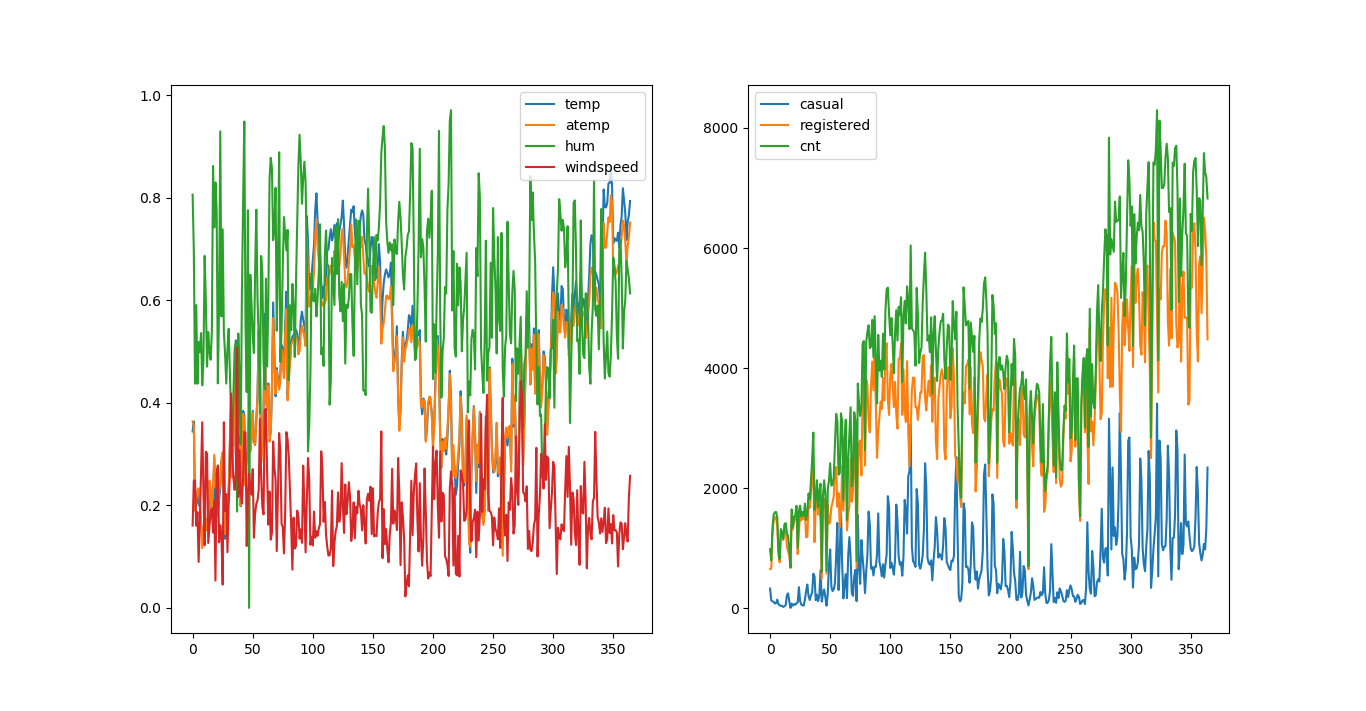
\includegraphics[width=.9\textwidth]{train-day}} \\
    \cprotect\subcaptionbox{\commandbox{hour.csv}训练集数据可视化\label{F:train-hour}}
        {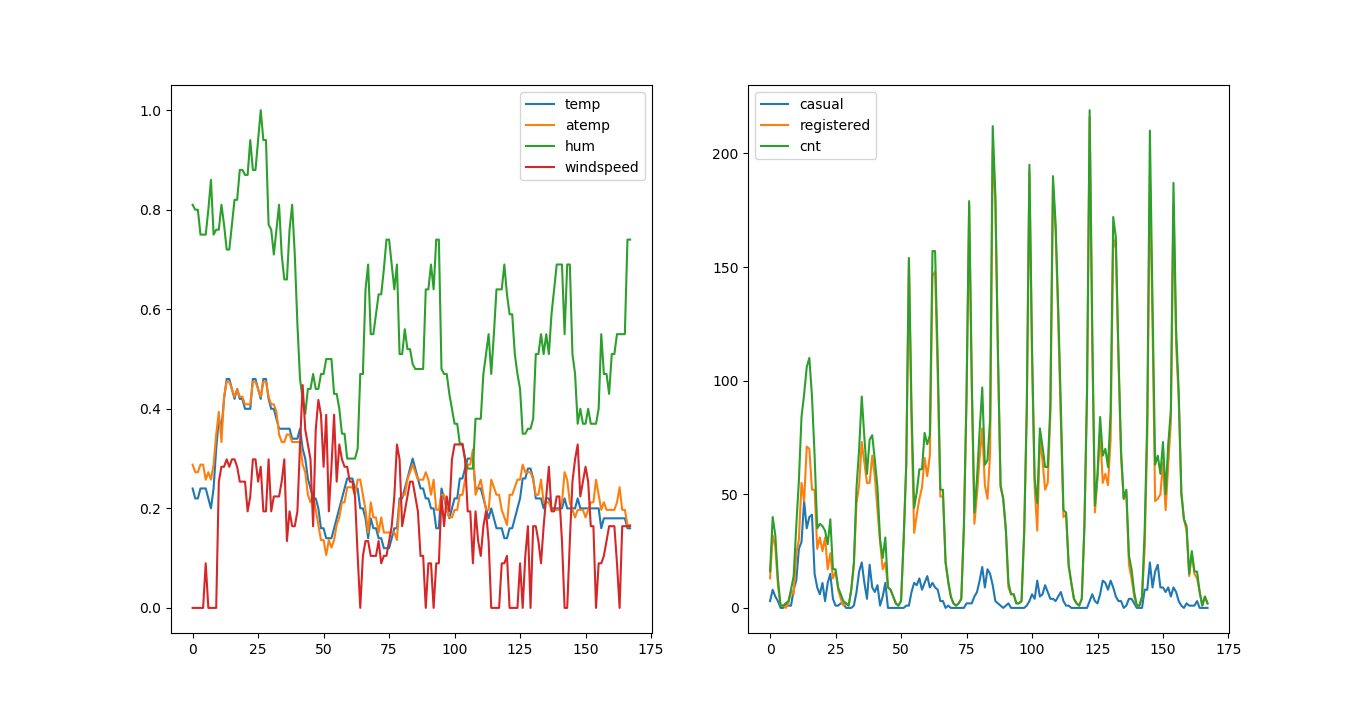
\includegraphics[width=.9\textwidth]{train-hour}}
    \caption{训练集数据可视化}\label{F:train}
\end{figure}

\subsubsection{测试集}
如图~\ref{F:test-day}与图~\ref{F:test-hour}可知,按照天数来说,用户数量的趋势与温度较为类似,而在小时尺度下则呈现不出明显的规律,有待于进一步的研究与建模。
\begin{figure}[htbp]
    \centering
    \cprotect\subcaptionbox{\commandbox{day.csv}测试集数据可视化\label{F:test-day}}
        {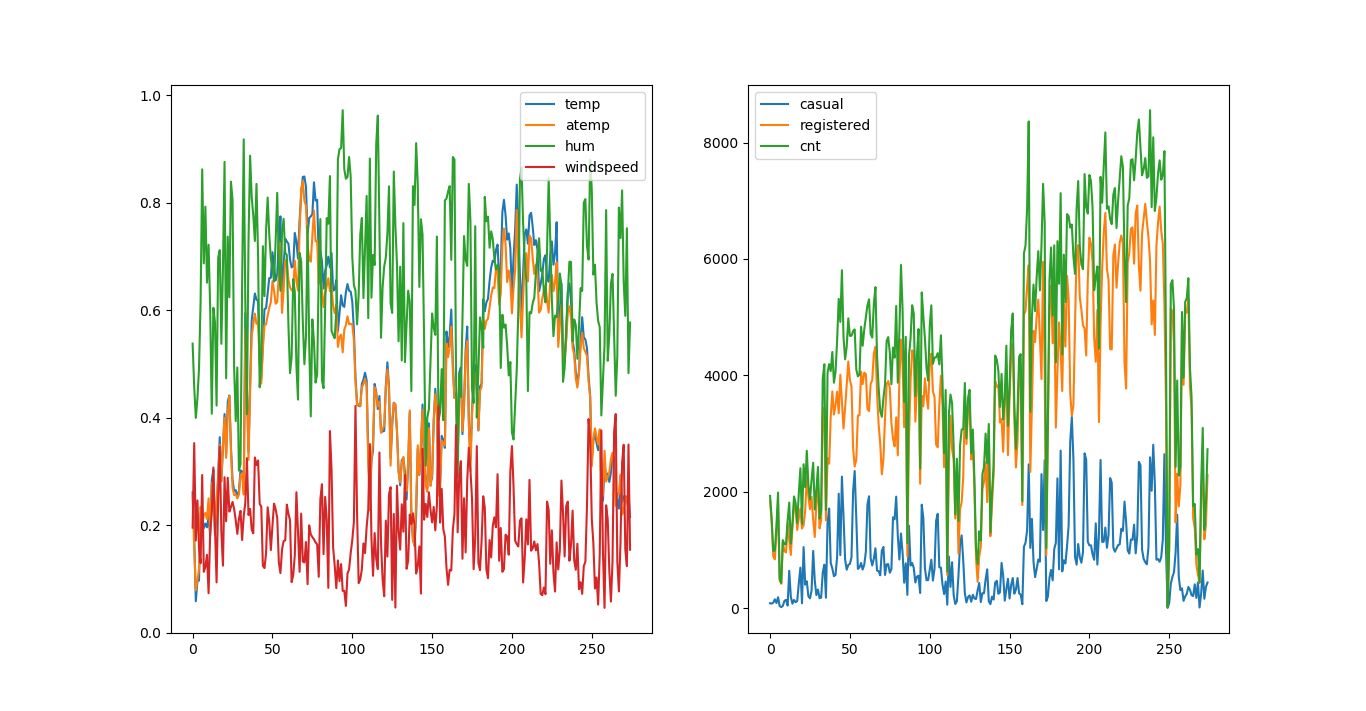
\includegraphics[width=.9\textwidth]{test-day}} \\
    \cprotect\subcaptionbox{\commandbox{hour.csv}测试集数据可视化\label{F:test-hour}}
        {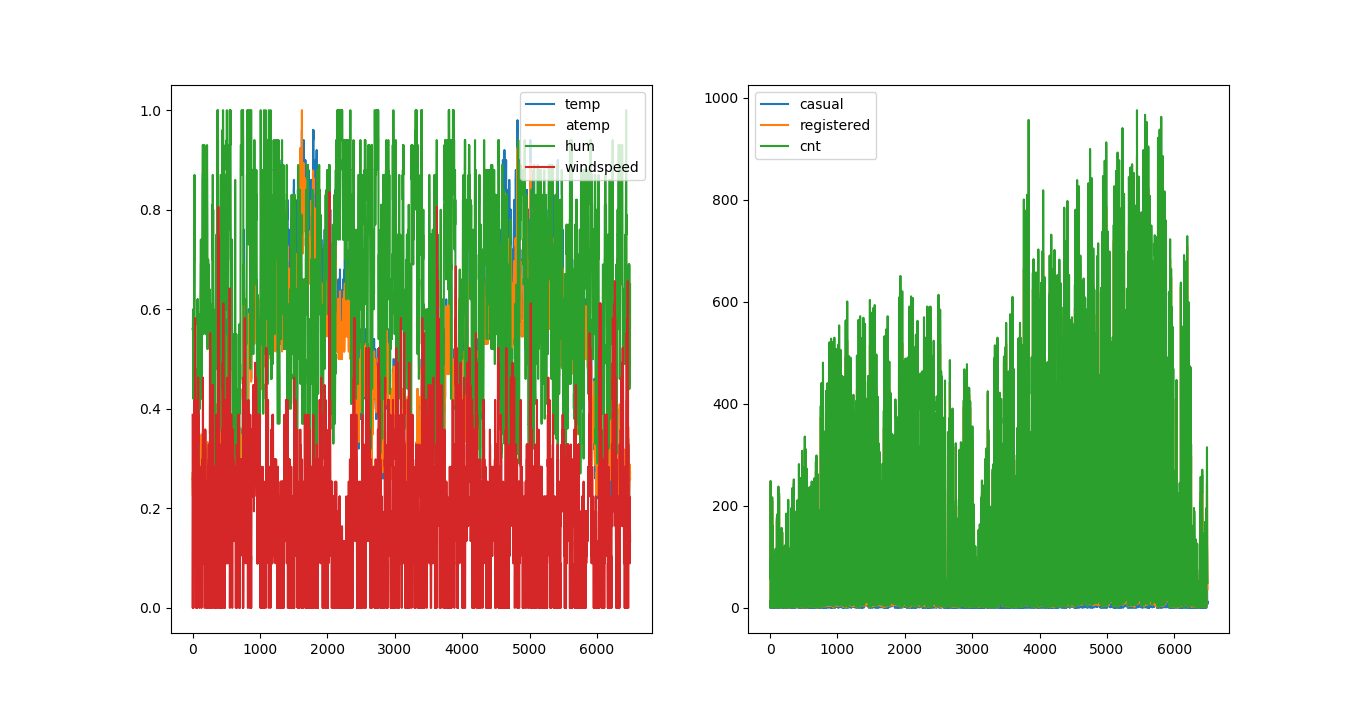
\includegraphics[width=.9\textwidth]{test-hour}}
    \caption{测试集数据可视化}\label{F:test}
\end{figure}

\subsubsection{时间相关变量数据集}
时间相关变量的训练集与测试集的数据趋势相差不大,因此我们只讨论训练集的数据可视化结果,如图~\ref{F:train-time}。

由图~\ref{F:train-time-hr}可知,不同颜色的线条对应着不同的时间点,而图中颜色呈现分层的效果,所以说用户数量与时间点之间存在较强的相关性。由图~\ref{F:train-time-mnth}与图~\ref{F:train-time-season}可知,2011年与2012年的数据呈现相似性,即大体趋势基本一致而对应月份的用户数量大致呈现倍数增加的关系。同时夏秋季节的用户数量多于春冬季节,符合温度对用户数量存在影响的假设。最后由图~\ref{F:train-time-workingday}可知,用户数量多的时间绝大部分为工作日,只有少数几天例外。
\begin{figure}[htbp]
    \centering
    \subcaptionbox{训练集上小时数与响应的关系图\label{F:train-time-hr}}
        {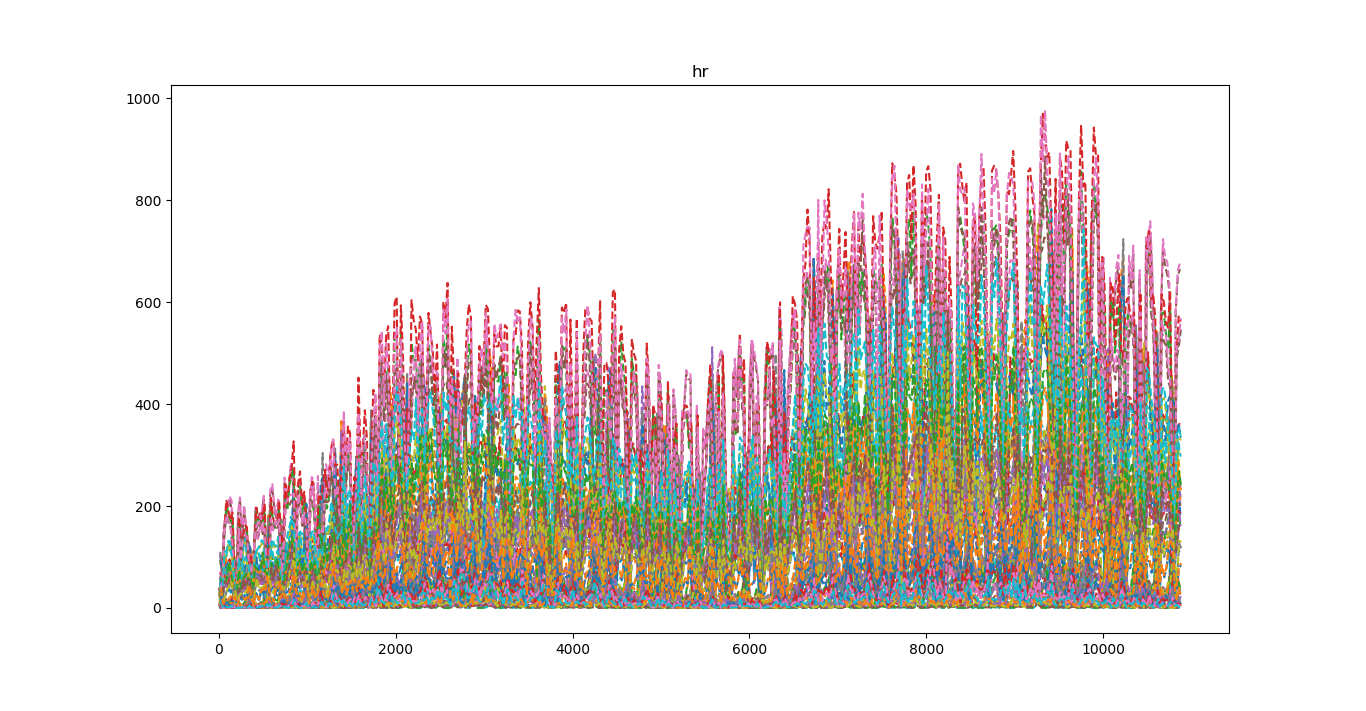
\includegraphics[width=.45\textwidth]{train-time-hr}}
    \subcaptionbox{训练集上月份与响应的关系图\label{F:train-time-mnth}}
        {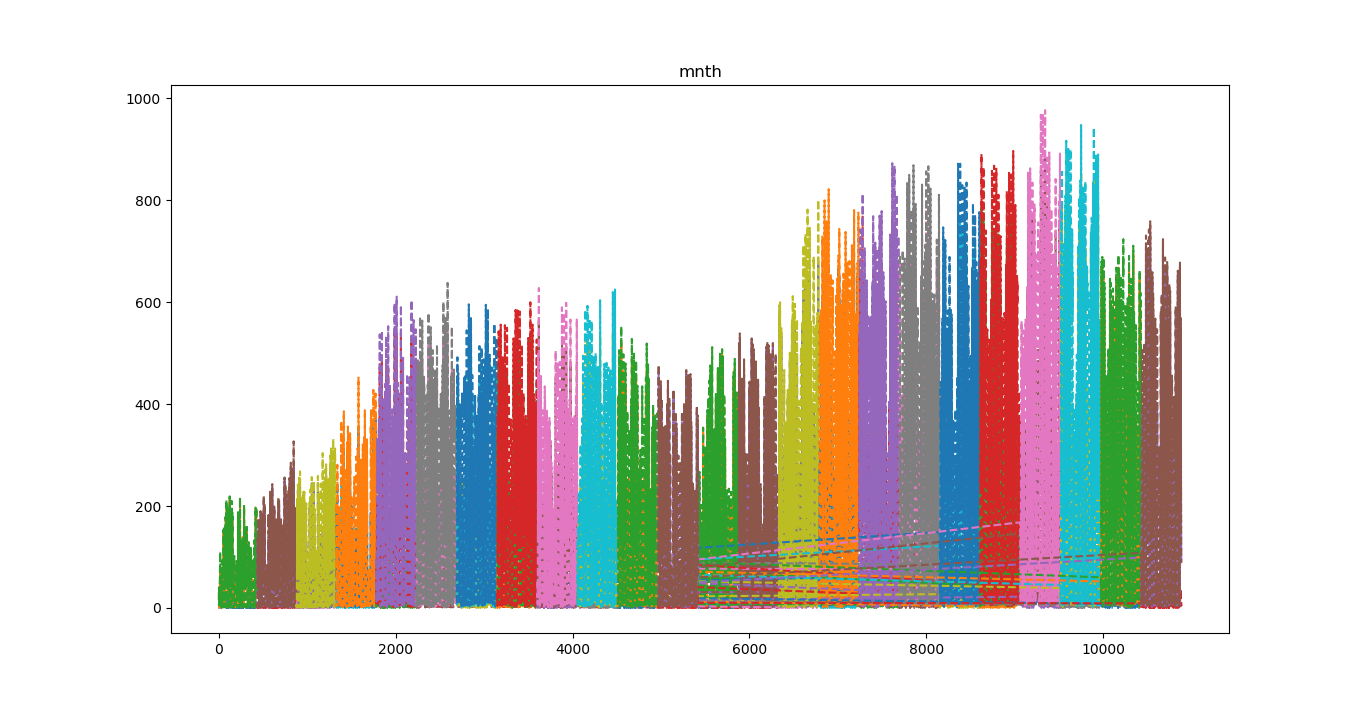
\includegraphics[width=.45\textwidth]{train-time-mnth}} \\
    \subcaptionbox{训练集上季节与响应的关系图\label{F:train-time-season}}
        {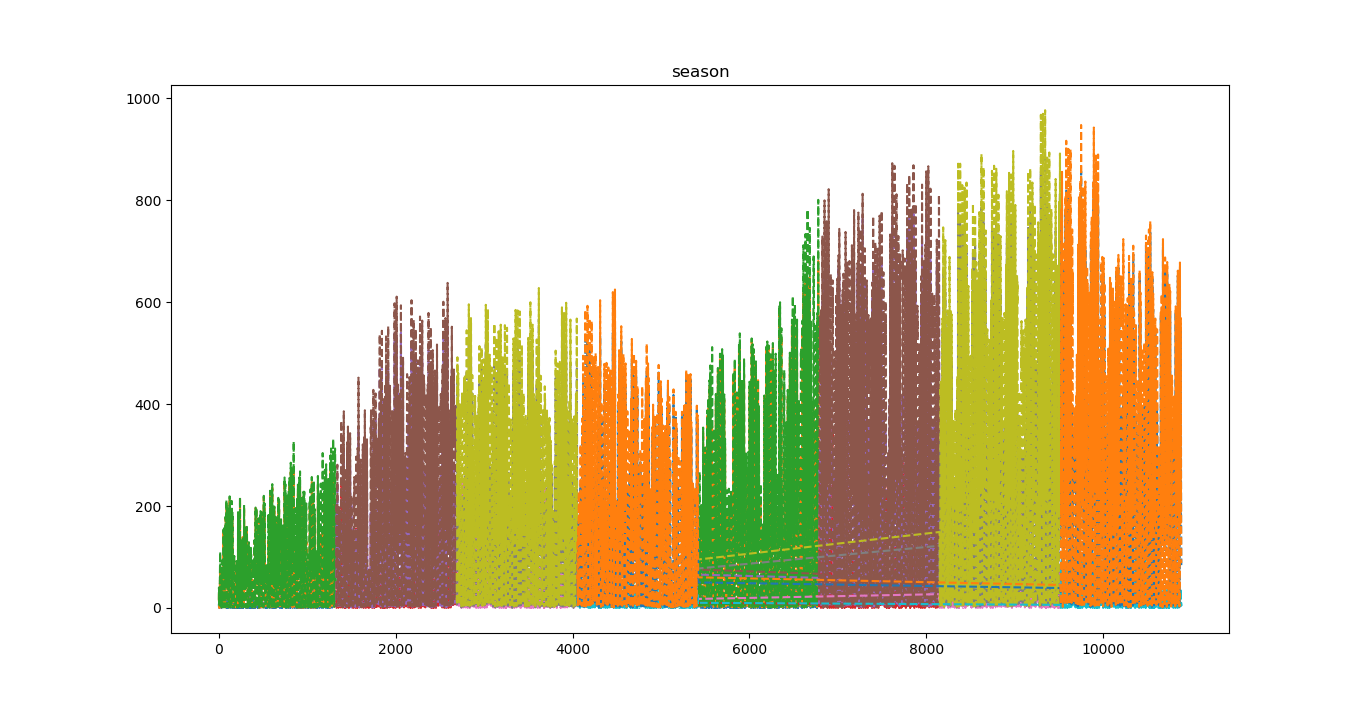
\includegraphics[width=.45\textwidth]{train-time-season}}
    \subcaptionbox{训练集上工作日与响应的关系图\label{F:train-time-workingday}}
        {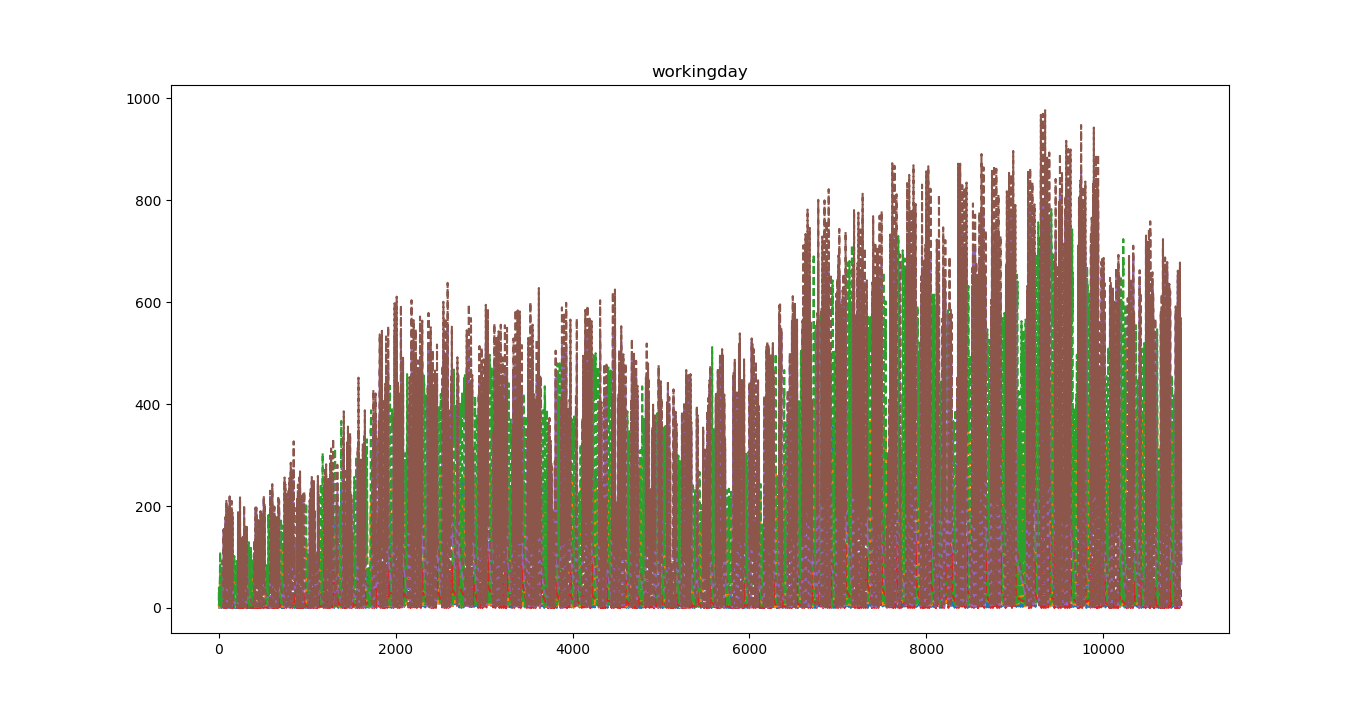
\includegraphics[width=.45\textwidth]{train-time-workingday}}
    \caption{训练集上时间有关变量与响应的关系图}\label{F:train-time}
\end{figure}

\begin{figure}[htbp]
    \centering
    \subcaptionbox{测试集上小时数与响应的关系图\label{F:test-time-hr}}
        {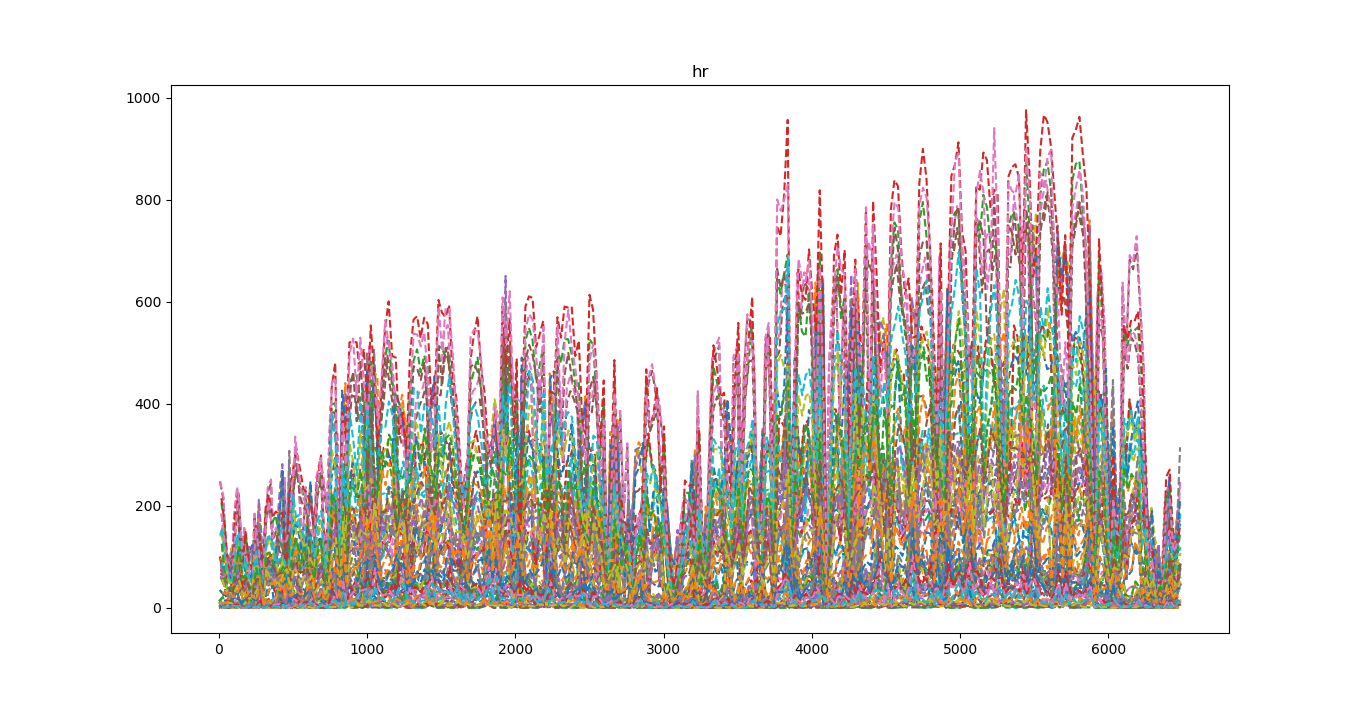
\includegraphics[width=.45\textwidth]{test-time-hr}}
    \subcaptionbox{测试集上月份与响应的关系图\label{F:test-time-mnth}}
        {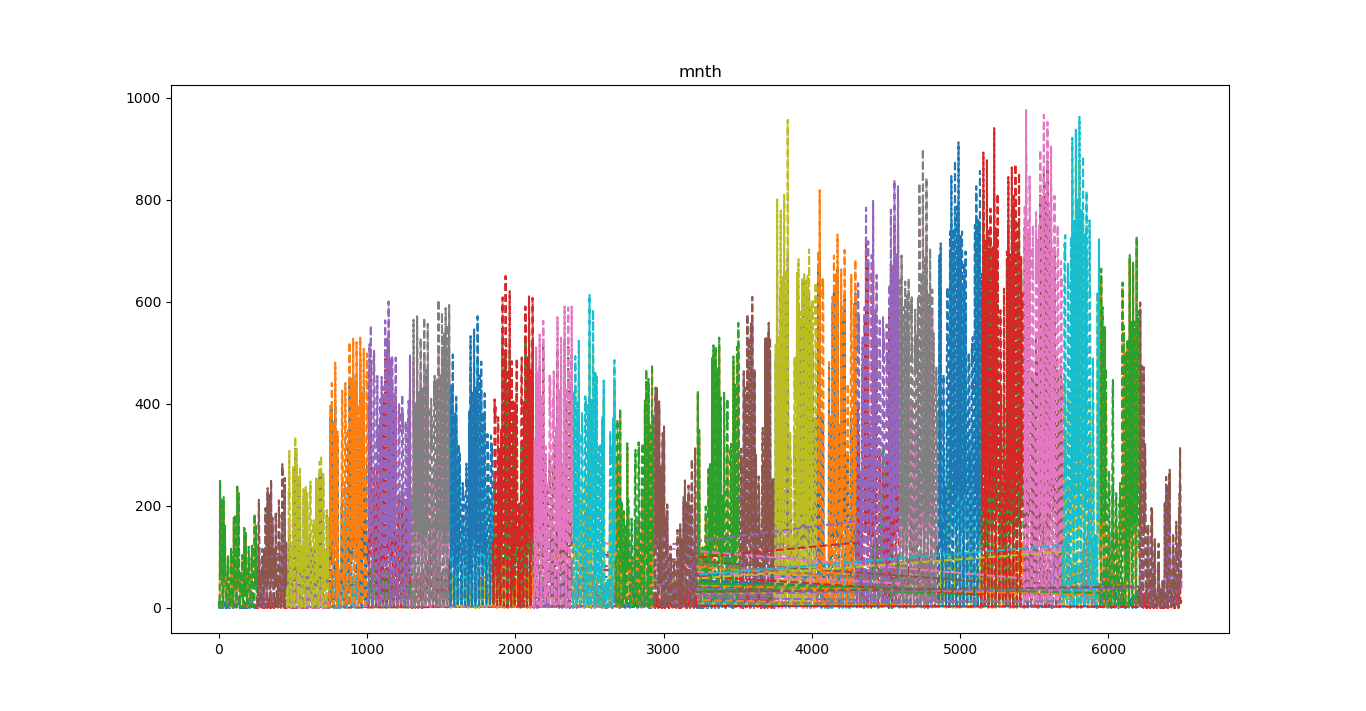
\includegraphics[width=.45\textwidth]{test-time-mnth}} \\
    \subcaptionbox{测试集上季节与响应的关系图\label{F:test-time-season}}
        {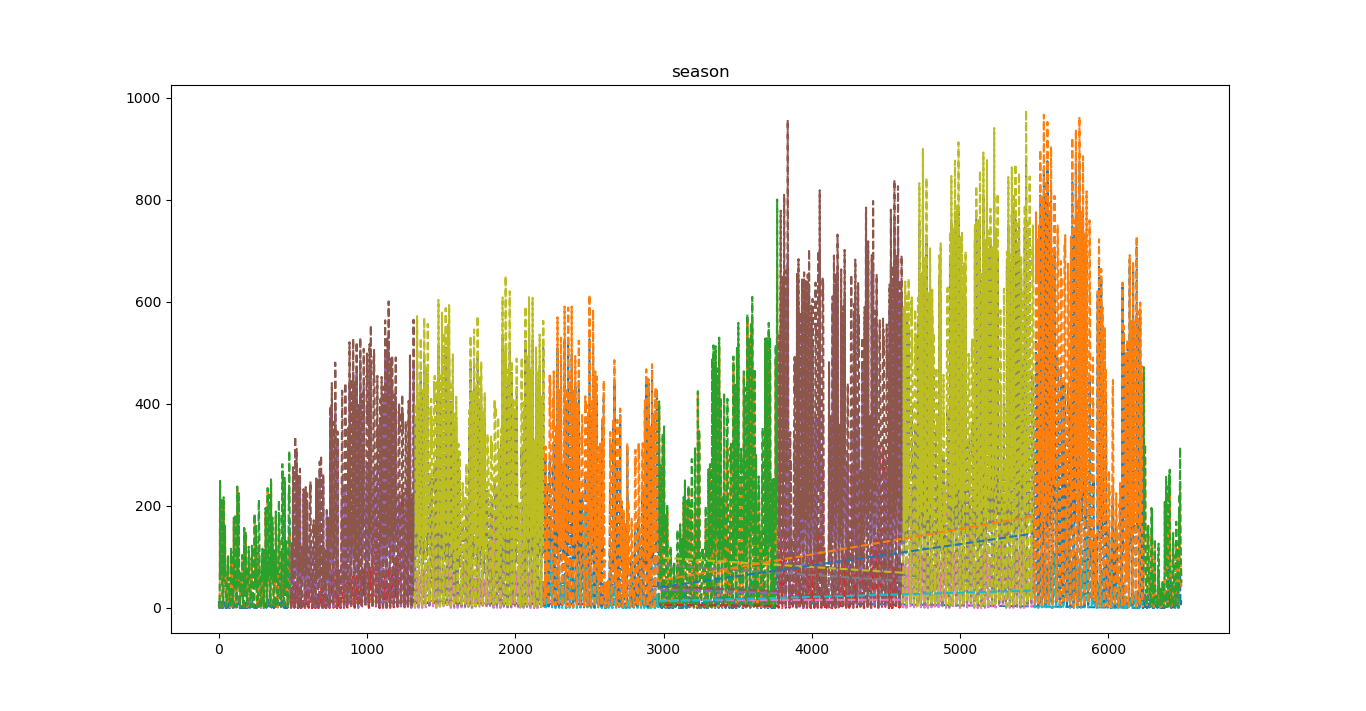
\includegraphics[width=.45\textwidth]{test-time-season}}
    \subcaptionbox{测试集上工作日与响应的关系图\label{F:test-time-workingday}}
        {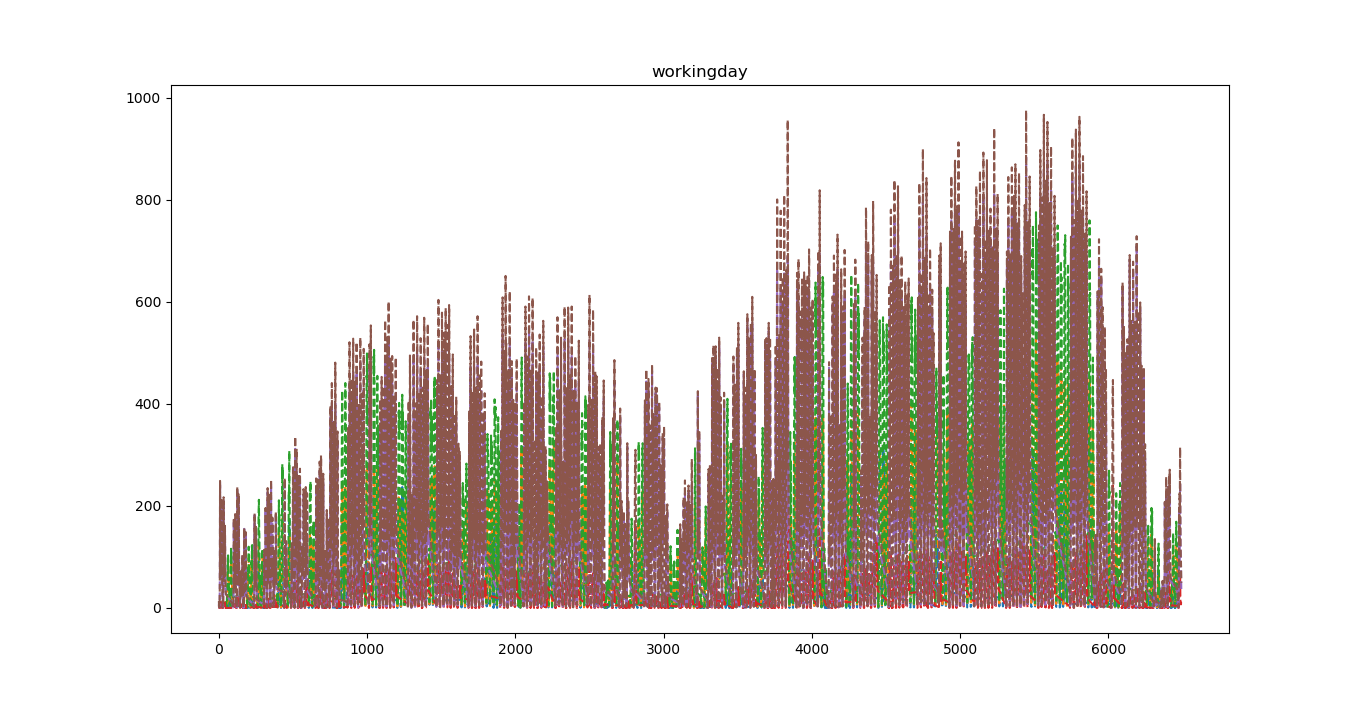
\includegraphics[width=.45\textwidth]{test-time-workingday}}
    \caption{测试集上时间有关变量与响应的关系图}\label{F:test-time}
\end{figure}
